%============================================
%                 ubuntu安装
%============================================
\subsection{Ubuntu安装}
\subsubsection{安装系统}
\begin{itemize}
\item Ubuntu系统镜像安装包链接:\url{https://pan.baidu.com/s/1rpWX2-Tb_MG5p93OJqLE4Q},提取码:9mbf
\item 使用u盘安装即可
\end{itemize}

\subsubsection{修改国内源}
\begin{itemize}
\item 备份原来文件
\begin{commandbox}
 > sudo cp /etc/apt/sources.list /etc/apt/sources.list_old
\end{commandbox}

\item 修改文件内容
\begin{commandbox}
 > sudo gedit /etc/apt/sources.list
\end{commandbox}
替换为\url{https://mirrors.tuna.tsinghua.edu.cn/help/ubuntu/}内容
\begin{messagebox}
# 默认注释了源码镜像以提高 apt update 速度,如有需要可自行取消注释
deb https://mirrors.tuna.tsinghua.edu.cn/ubuntu/ xenial main restricted universe multiverse
# deb-src https://mirrors.tuna.tsinghua.edu.cn/ubuntu/ xenial main restricted universe multiverse
deb https://mirrors.tuna.tsinghua.edu.cn/ubuntu/ xenial-updates main restricted universe multiverse
# deb-src https://mirrors.tuna.tsinghua.edu.cn/ubuntu/ xenial-updates main restricted universe multiverse
deb https://mirrors.tuna.tsinghua.edu.cn/ubuntu/ xenial-backports main restricted universe multiverse
# deb-src https://mirrors.tuna.tsinghua.edu.cn/ubuntu/ xenial-backports main restricted universe multiverse
deb https://mirrors.tuna.tsinghua.edu.cn/ubuntu/ xenial-security main restricted universe multiverse
# deb-src https://mirrors.tuna.tsinghua.edu.cn/ubuntu/ xenial-security main restricted universe multiverse

# 预发布软件源,不建议启用
# deb https://mirrors.tuna.tsinghua.edu.cn/ubuntu/ xenial-proposed main restricted universe multiverse
# deb-src https://mirrors.tuna.tsinghua.edu.cn/ubuntu/ xenial-proposed main restricted universe multiverse
\end{messagebox}

\begin{messagebox}
deb http://mirrors.aliyun.com/ubuntu/ focal main restricted universe multiverse
deb http://mirrors.aliyun.com/ubuntu/ focal-security main restricted universe multiverse
deb http://mirrors.aliyun.com/ubuntu/ focal-updates main restricted universe multiverse
deb http://mirrors.aliyun.com/ubuntu/ focal-proposed main restricted universe multiverse
deb http://mirrors.aliyun.com/ubuntu/ focal-backports main restricted universe multiverse
deb-src http://mirrors.aliyun.com/ubuntu/ focal main restricted universe multiverse
deb-src http://mirrors.aliyun.com/ubuntu/ focal-security main restricted universe multiverse
deb-src http://mirrors.aliyun.com/ubuntu/ focal-updates main restricted universe multiverse
deb-src http://mirrors.aliyun.com/ubuntu/ focal-proposed main restricted universe multiverse
deb-src http://mirrors.aliyun.com/ubuntu/ focal-backports main restricted universe multiverse

deb https://mirrors.tuna.tsinghua.edu.cn/ubuntu/ eoan main restricted universe multiverse
deb-src https://mirrors.tuna.tsinghua.edu.cn/ubuntu/ eoan main restricted universe multiverse
deb https://mirrors.tuna.tsinghua.edu.cn/ubuntu/ eoan-updates main restricted universe multiverse
deb-src https://mirrors.tuna.tsinghua.edu.cn/ubuntu/ eoan-updates main restricted universe multiverse
deb https://mirrors.tuna.tsinghua.edu.cn/ubuntu/ eoan-backports main restricted universe multiverse
deb-src https://mirrors.tuna.tsinghua.edu.cn/ubuntu/ eoan-backports main restricted universe multiverse
deb https://mirrors.tuna.tsinghua.edu.cn/ubuntu/ eoan-security main restricted universe multiverse
deb-src https://mirrors.tuna.tsinghua.edu.cn/ubuntu/ eoan-security main restricted universe multiverse
deb https://mirrors.tuna.tsinghua.edu.cn/ubuntu/ eoan-proposed main restricted universe multiverse
deb-src https://mirrors.tuna.tsinghua.edu.cn/ubuntu/ eoan-proposed main restricted universe multiverse
\end{messagebox}

\item 更新软件列表
\begin{commandbox}
 > sudo apt update
 > sudo apt upgrade
\end{commandbox}

\end{itemize}

\subsubsection{ubuntu16.04配置vnc远程控制环境}
\begin{itemize}
\item 在系统搜索\emphasizebox{desktop}
\begin{figure}[H]
\centering
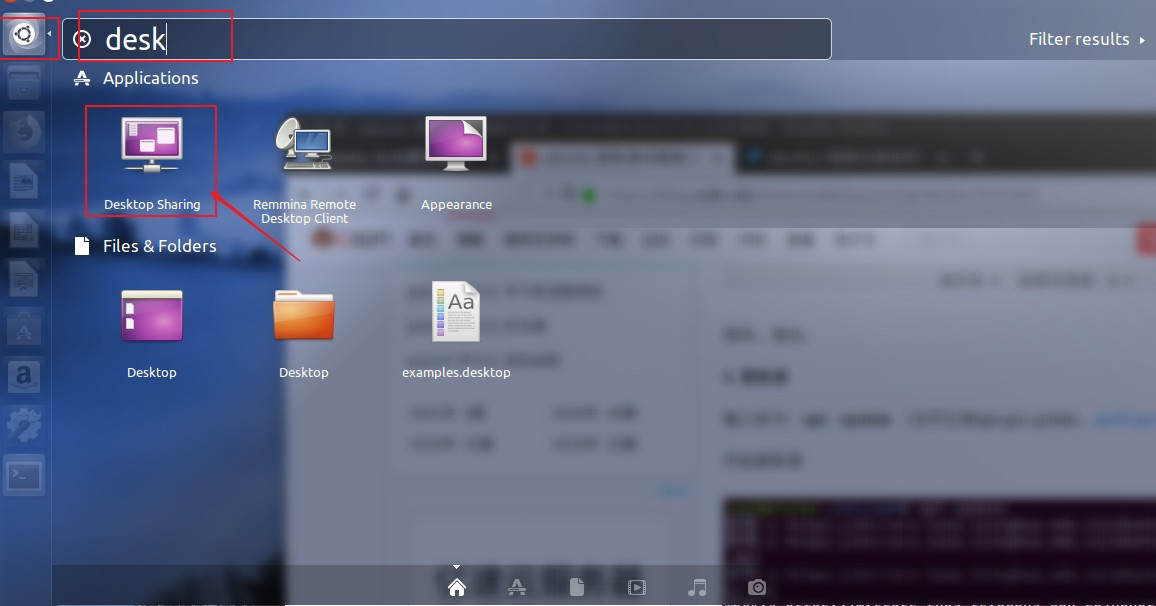
\includegraphics[scale=0.5]{001_desktop_share.jpg}
\caption{点击desktop\_sharing}
\end{figure}

\item 配置为下图所示
\begin{figure}[H]
\centering
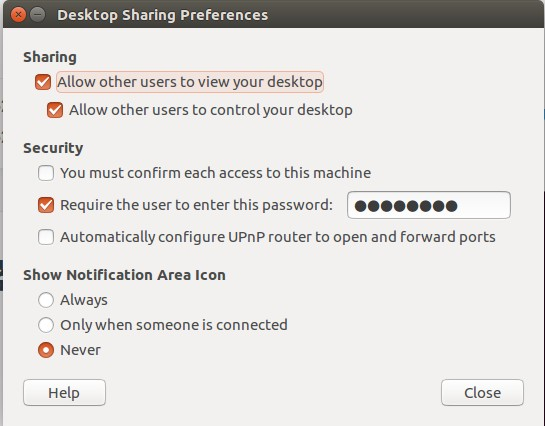
\includegraphics[scale=0.7]{002_desktop_share_config.jpg}
\caption{配置如图}
\end{figure}

\item 安装vncserver
\begin{commandbox}
 > sudo apt-get install xrdp vnc4server xbase-clients
\end{commandbox}

\item 安装dconf-editor(取消权限限制)
\begin{commandbox}
 > sudo apt-get install dconf-editor
\end{commandbox}

\item 搜索打开dconf-editor
\begin{figure}[H]
\centering
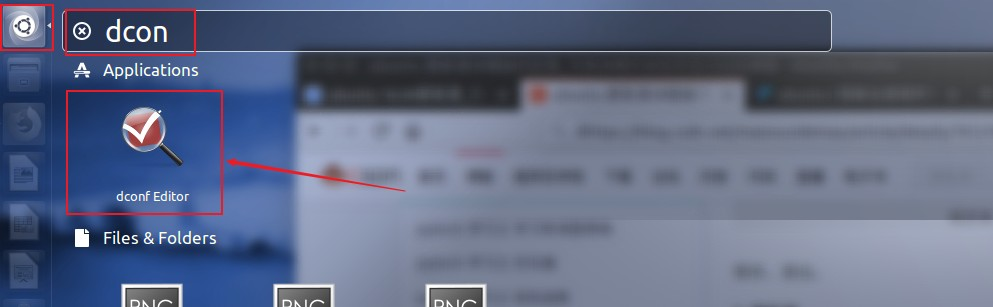
\includegraphics[scale=0.5]{003_dconf_editor.jpg}
\caption{点击dconf-editor}
\end{figure}

\item 配置dconf-editor如下图, 路径:
\begin{messagebox}
org->gnome->desktop->remote-access
\end{messagebox}

\begin{figure}[H]
\centering
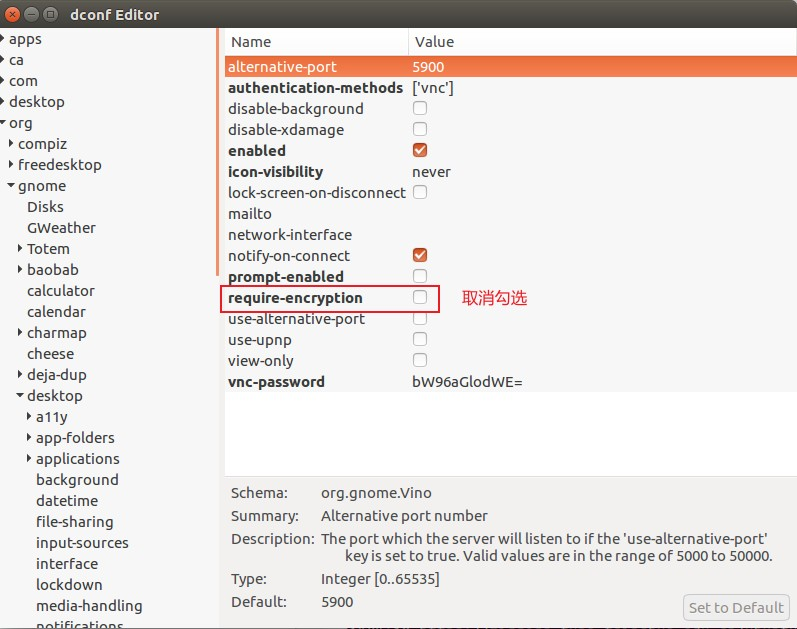
\includegraphics[scale=0.7]{004_dconf_editor_config.jpg}
\caption{配置如图dconf-editor}
\end{figure}

\item 电脑端使用vnc软件连接即可。

\end{itemize}

%============================================
%         ubuntu20.04配置VNC远程登陆环境
%============================================
\subsubsection{ubuntu20.04配置vnc远程控制环境}
\begin{itemize}

\item 在系统设置里面,点击\emphasizebox{共享} --> \emphasizebox{屏幕共享}
\begin{figure}[H]
\centering
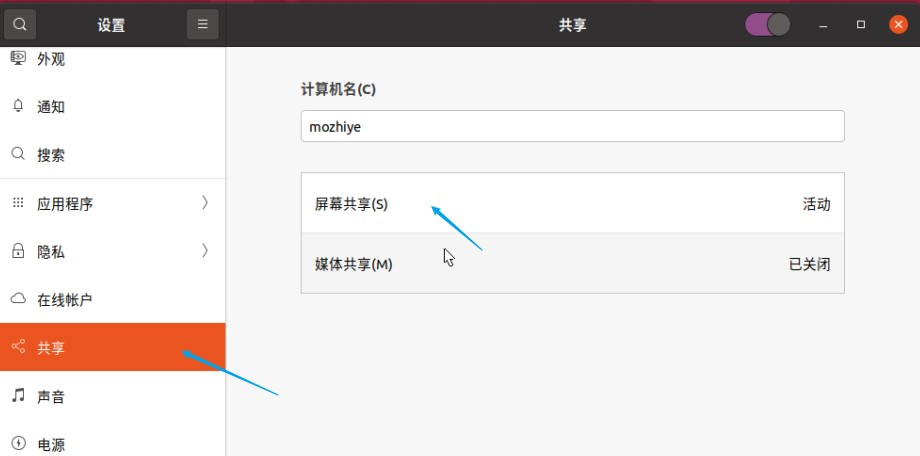
\includegraphics[scale=0.5]{005_20_04_desktop_set.jpg}
\caption{共享设置}
\end{figure}

\item 设置为如图
\begin{figure}[H]
\centering
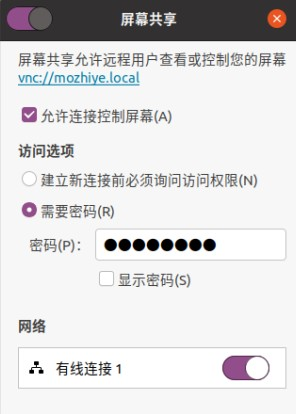
\includegraphics[scale=0.5]{006_20_04_desktop_set_step2.jpg}
\caption{配置为图中所示}
\end{figure}

\item 安装dconf-editor(取消权限限制)
\begin{commandbox}
# 安装dconf-editor
 > sudo apt-get install dconf-editor
\end{commandbox}

\item 搜索打开dconf-editor, 配置dconf-editor如下图, 路径:
\begin{messagebox}
org->gnome->desktop->remote-access
\end{messagebox}
\begin{figure}[H]
\centering
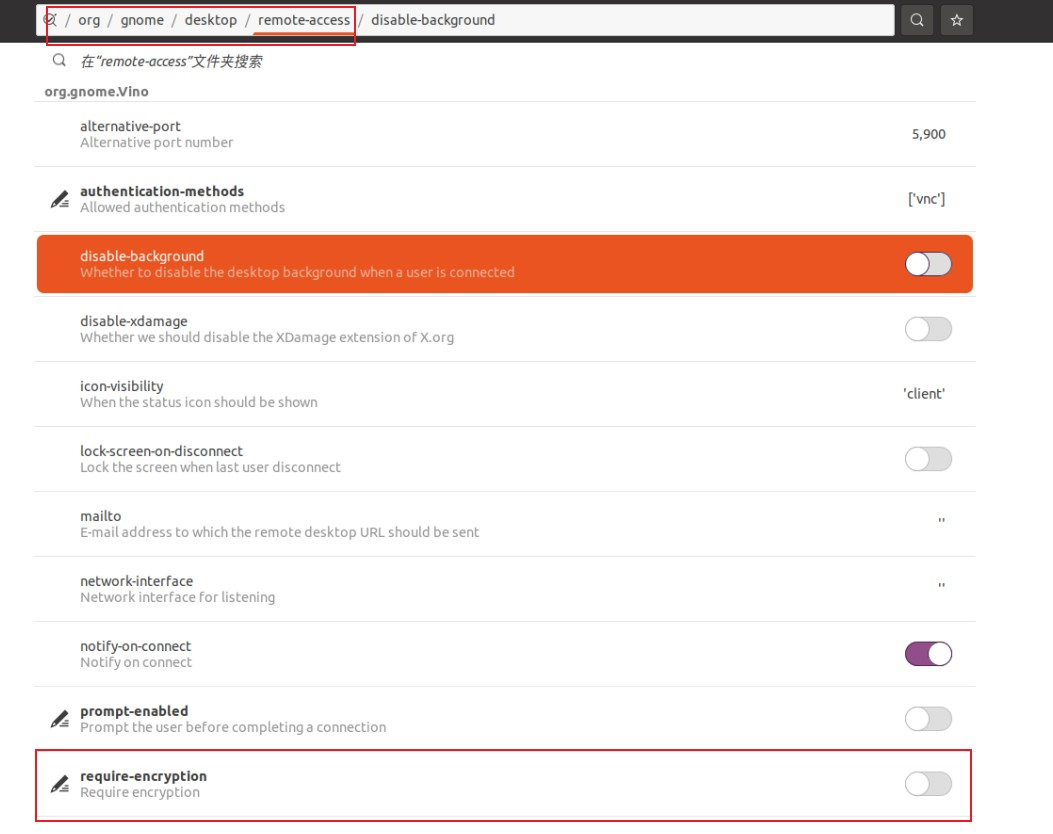
\includegraphics[scale=0.5]{007_20_04_desktop_set_step3.jpg}
\caption{配置如图dconf-editor}
\end{figure}

\item 电脑端使用vnc软件连接即可。

\end{itemize}

%============================================
%           配置ssh远程登陆环境
%============================================
\subsubsection{配置ssh远程登陆环境}
\begin{itemize}
\item 查看ssh是否安装
\begin{commandbox}
 > sudo sudo ps -e | grep ssh
\end{commandbox}
如果什么信息都没有,证明没安装

\item 安装ssh
\begin{commandbox}
 > sudo apt-get install openssh-server
\end{commandbox}

\item 查看配置文件,查看端口号是不是22
\begin{commandbox}
 > vim /etc/ssh/sshd_config
\end{commandbox}

\item 使用ssh软件登陆即可。

\end{itemize}

%============================================
%           配置samba共享文件系统
%============================================
\subsubsection{配置samba共享文件系统}
\begin{itemize}
\item 安装samba
\begin{commandbox}
 > sudo apt-get install samba
\end{commandbox}

\item 配置smb.conf文件
\begin{commandbox}
 > sudo gedit /etc/samba/smb.conf
\end{commandbox}
在最后添加如下信息, 其中work为对外显示的文件夹名称, 访问用户名为mozhiye
\begin{messagebox}
[work]
    comment = samba home directory 
    path = /home/mozhiye/100_share_dir
    public = yes
    browseable = yes
    public = yes
    read only = no
    valid users = mozhiye
    create mask = 0777
    directory mask = 0777 
    force user = nobody
    force group = nogroup
    available = yes
\end{messagebox}

\item 增加登陆用户名密码
\begin{commandbox}
 > sudo smbpasswd -a mozhiye
\end{commandbox}
输入密码即可

\item 创建共享文件夹
\begin{commandbox}
 > mkdir /home/mozhiye/100_share_dir
 > chmod 777 /home/mozhiye/100_share_dir
\end{commandbox}

\item 重启samba
\begin{commandbox}
 > sudo service smbd restart
\end{commandbox}

\item WINDOWS端输入IP访问即可。
\end{itemize}

%============================================
%           安装git
%============================================
\subsubsection{安装git}
\begin{itemize}
\item 安装git
\begin{commandbox}
 > sudo apt-get instal git
\end{commandbox}

\item 参考git配置章节配置git环境
\end{itemize}

%============================================
%       使用LINUX_TOOLS配置bash和vim
%============================================
\subsubsection{使用LINUX\_TOOLS配置bash和vim}
下载LINUX\_TOOLS文件夹放到根目录,todo:补路径, \emphasizebox{注意}先要预先安装所需软件, 后通过LINUX\_TOOLS覆盖配置
\begin{itemize}

\item 安装git

\item 安装vim
\begin{commandbox}
 > sudo apt-get instal vim
\end{commandbox}

\item 安装cscope
\begin{commandbox}
 > sudo apt-get instal cscope
\end{commandbox}

\item 安装ctags
\begin{commandbox}
 > sudo apt-get instal ctags
\end{commandbox}

\item 安装zsh
\begin{commandbox}
 > sudo apt-get instal zsh
\end{commandbox}

\item 安装oh-my-zsh, 进入LINUX\_TOOLS/oh-my-zsh\_installl/tools目录
\begin{commandbox}
 > sh install.sh
\end{commandbox}

\item 修改默认登陆shell
\begin{commandbox}
 > chsh -s /bin/zsh
\end{commandbox}

\item 运行LINUX\_TOOLS里面的安装命令

\item 退出ssh,重新登陆

\item 测试c语言工程插件是否会出错

\item TODO:研究vim复制粘贴板问题
\end{itemize}


%============================================
%           关闭自动锁屏
%============================================
\subsubsection{关闭自动锁屏和登陆输入密码}

%============================================
%           安装文件传输命令rz sz
%============================================
\subsubsection{安装文件传输命令rz/sz}
\begin{commandbox}
 > sudo apt-get install lrzsz
\end{commandbox}

%============================================
%           安装latex
%============================================
\subsubsection{安装latex}
\begin{commandbox}
 > sudo apt-get install texlive-full
\end{commandbox}
使用latex工程测试环境

\begin{itemize}
    \item 使用\emphasizebox{Crtl + D}中断编译过程
    \item 使用\emphasizebox{evince}可以打开pdf文件
    \item 怎么使用系统字体, 用命令生成文件查看字体族: 查看latex字体搜索范围
\begin{commandbox}
 > vim /usr/share/texlive/texmf-dist/web2c/texmf.cnf
\end{commandbox}

查看变量
\begin{messagebox}
% OSFONTDIR is to provide a convenient hook for allowing TeX to find
% fonts installed on the system (outside of TeX).  An empty default
% value would add "//" to the search paths, so we give it a dummy value.
OSFONTDIR = /usr/share/fonts
\end{messagebox}

\begin{commandbox}
fc-list > font_list列出所有(输出显示格式为: 字体族中文名,字体族英文名:变体)
fc-list :lang=zh > font_ch_list 列出中文字体
fc-list -f "%{family}\n" > font_family_list 只列出字体族名
\end{commandbox}
把命令保存为文件, 在font\_family\_list文件中查看可以使用的系统字体族

\end{itemize}

%============================================
%           安装ubuntu自定义字体
%============================================
\subsubsection{安装ubuntu自定义字体}
\begin{itemize}
\item 在win10系统复制字体tff文件

\item  在linux路径
\begin{messagebox}
/usr/share/fonts/
\end{messagebox}
新建文件夹
\begin{messagebox}
/usr/share/fonts/winfonts/consolas
把tff文件复制到该目录
\end{messagebox}

\item 改变tff文件权限
\begin{commandbox}
sudo chmod 644 /usr/share/fonts/winFonts/*.ttf
\end{commandbox}

\item 创建字体的fonts.scale文件,它用来控制字体旋转缩放
\begin{commandbox}
sudo mkfontscale
\end{commandbox}

\item 创建雅黑字体的fonts.dir文件,它用来控制字体粗斜体产生
\begin{commandbox}
sudo mkfontdir
\end{commandbox}

\item 建立字体缓存信息,也就是让系统认识新安装字体
\begin{commandbox}
sudo fc-cache -fv
\end{commandbox}

\item 在latex章节用fc-list命令查看字节是否安装

\end{itemize}

%============================================
%           安装make
%============================================
\subsubsection{安装make}
\begin{commandbox}
 > sudo apt-get install make
\end{commandbox}

%============================================
%           安装meld
%============================================
\subsubsection{安装make}
\begin{commandbox}
 > sudo apt-get install meld
\end{commandbox}
